Segundo Ahmad et al.~\cite{ahmad2015automatic}, o reconhecimento de placas
automotivas requer três passos, a localização da placa, a separação dos
caracteres e o reconhecimento dos caracteres. S Du~\cite{s2013automatic} ainda
defende que são nescessários os mesmos passos, com a inclusão da aquisição das
imagens como passo inicial. Para a localização da placa e separação dos
caracteres serão utilizadas a biblioteca OpenCV e a linguagem de programação
Python. O motivo da escolha dessa linguagem se dá por ser uma das linguagens
mais usadas para OpenCV\@. Para o reconhecimento dos caracteres será utilizado o
software Tesseract, havendo a possibilidade de precisar ser treinado para
reconhecer a fonte da placa de transito brasileira. As escolhas a serem feitas
tem como objetivo maximizar os resultados ao final do trabalho, tentando criar
um balanço entre facilidade de implementação e qualidade do reconhecimento.

\begin{figure}[H]
	\centering
	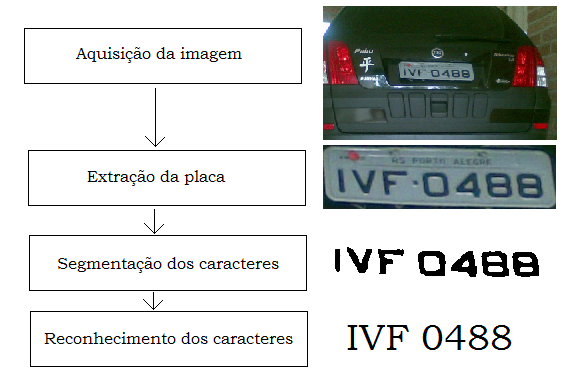
\includegraphics[width=88mm]{processo.png}
	\caption{Quatro estágios do reconhecimento de placa}
	\label{fig:processo}
\end{figure}

O trabalho será dividido nos quatro passos propostos por S
Du~\cite{s2013automatic}: aquisição da imagem, extração da placa, segmentação
dos caracteres e reconhecimento dos caracteres.

\section{Aquisição das imagens}
\label{sec:aquisicao}

O primeiro passo para o reconhecimento de uma placa é a extração das imagens,
que é um passo simples porém importante do reconhecimento. Diversos fatores
externos podem afetar o reconhecimento da placa, como a iluminação, a distância
e o ângulo da imagem. A influência desses fatores pode ser minimizada
utilizando-se de imagens de qualidade.

A aquisição das imagens será feita utilizando o módulo de câmera do
\emph{Raspberry Pi}. É uma câmera de 5 \emph{megapixels} capaz de gravar videos
em 1080p. Uma das vantagens de utilizar essa combinação do \emph{Raspberry Pi} e
seu módulo de câmera é a sua portabilidade. Por serem pequenos e leves, caso a
câmera tenha dificuldade em capturar imagens de qualidade para o reconhecimento
das placas, é possível movê-los e colocá-los em posições privilegiadas para
otimizar o processo.

\section{Extração da placa}
\label{sec:extracao}

A fase de extração é a fase mais importante em um sistema de reconhecimento de
placas, porque todas as outras fases dependem da exata extração da área da
placa. Essa extração é difícil pois influencia na precisão do sistema como um
todo~\cite{kaur2014efficient}. Muitas dificuldades podem ocorrer durante a fase
de extração pelos seguintes motivos:

\begin{itemize}
	\item A eficiência da extração é afetada pela complexidade da cena.
	\item Diferentes veículos possuem suas placas em diferentes posições.
	\item Pode ocorrer ruído durante a captura da câmera.
	\item Condições do tempo pode influenciar no ruído.
	\item Hora do dia afeta na luminosidade e resulta em erros de contraste.
	\item Outros caracteres, quadros e parafusos podem introduzir confusão.
	\item Mal posicionamento da câmera, ou placa, pode resultar em distorção que afeta na eficiência.
	\item Luminosidade baixa, ou desigual, imagem desfocada, baixa resolução, reflexão, sombra afetam a eficiência da extração.
\end{itemize}

Kaur~\cite{kaur2014efficient} propõe um método eficiênte de
extração que segue o seguinte fluxograma:

\begin{enumerate}
	\item Aquisição de Imagem
	\item Conversão de RGB para escala de tons de cinza
	\item Remoção de ruído por filtro bilateral
	\item Aumento de contraste usando equalização de histograma adaptativo
	\item Operações Morfológicas de Abertura e Subtração de Imagem
	\item Binarização da Imagem
	\item Detecção de borda pelo operador Sobel
	\item Detecção de Área de Placa Candidata por Operações Morfológicas de Abertura e Fechamento
	\item Extração da área da placa real
	\item Aprimoramento da região extraída
\end{enumerate}

\section{Aquisição da imagem}

O primeiro passo é adquirir a imagem que vai servir de entrada. Essa imagem, no
contexto do nosso trabalho, vai vir de uma câmera digital ligada ao Raspberry
Pi.

\begin{figure}[H]
	\centering
	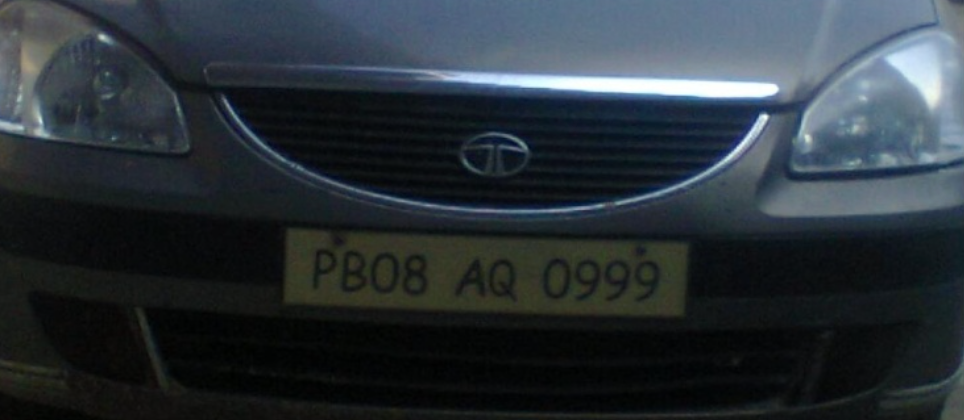
\includegraphics[width=88mm]{ext01.png}
	\caption{Imagem de entrada}
Fonte: An efficient approach for number plate extraction from vehicles image under image processing~\cite{kaur2014efficient}
	\label{fig:ext_input_image}
\end{figure}

\subsection{Pré-processamento}

O objetivo básico do pré-processamento é melhorar o contraste da imagem de
entrada, para reduzir ruído e, em consequência, a velocidade de
processamento. O melhoramento do contraste é feito pela equalização do
histograma, alongamento de contraste etc. Varios filtros são usados para a
remoção de ruído.

\subsection{Conversão de RGB para escala de tons de cinza}

A imagem capturada está no formato RGB\@. O primeiro passo do pré-processamento é
converter essa imagem para a escala de tons de cinza. O objetivo dessa conversão é reduzir
o número de cores. Os componentes R, G e B são separados do valor de cor de 24
bits de cada pixel (i,j), e um valor de 8 bits em cinza é calculado.

\begin{figure}[H]
	\centering
	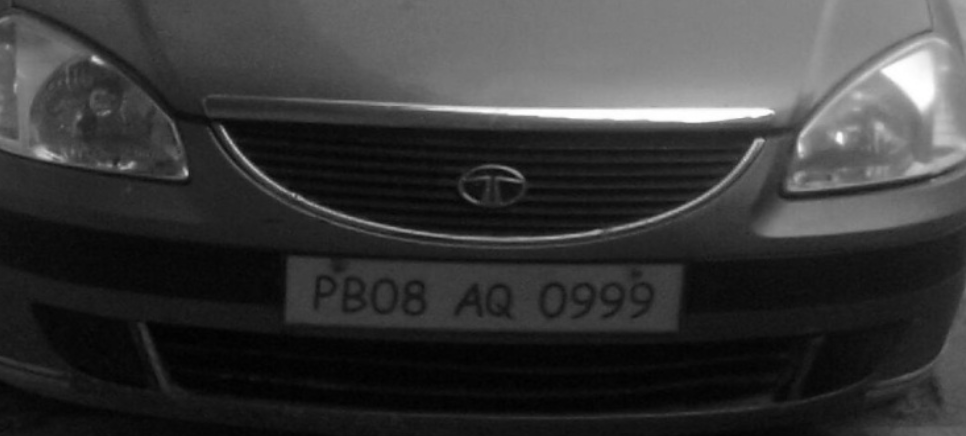
\includegraphics[width=88mm]{ext02.png}
	\caption{Imagem em escala de tons de cinza}
Fonte: An efficient approach for number plate extraction from vehicles image under image processing~\cite{kaur2014efficient}
	\label{fig:ext_gray_scale}
\end{figure}

\subsection{Remoção de ruído por filtro bilateral}

O filtro bilateral é um filtro não linear, que preserva as arestas e reduz ruído.
Ele funciona substituindo o valor de intensidade de cada \emph{pixel} em uma imagem
por uma média ponderada dos valores de intensidade dos \emph{pixels} próximos.
O objetivo básico da filtragem é remover ruído e distorção da imagem. O ruído
pode ocorrer durante a captura pela câmera ou pelas condições do tempo. No
método que Kaur~\cite{kaur2014efficient} propõe, filtro bilateral iterativo é
utilizado para remover ruído. Ele é não linear, provê mecanismo para remoção de
ruído enquanto preserva bordas mais efetifamente que o filtro mediano. O filtro
mediano funciona substituindo o valor de cada \emph{pixel} pela mediana dos \emph{pixels}
vizinhos.

\begin{figure}[H]
	\centering
	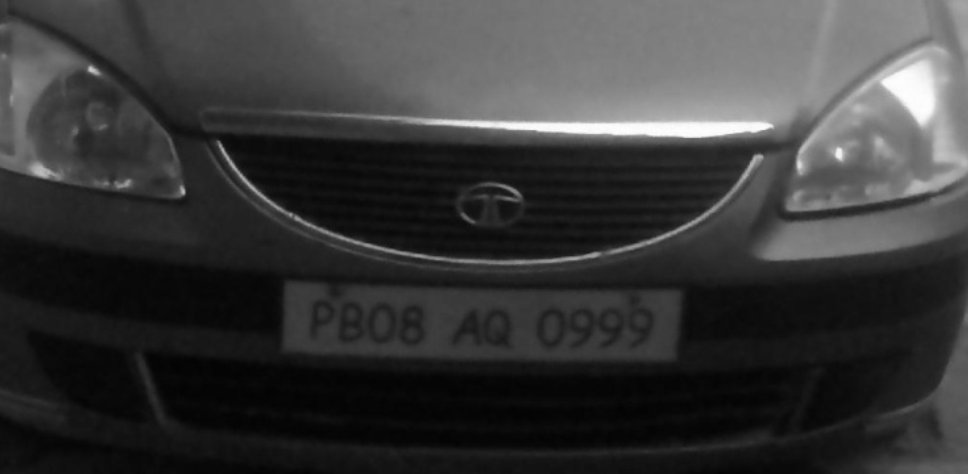
\includegraphics[width=88mm]{ext03.png}
	\caption{Aplicação de filtro bilateral em uma imagem em escala de tons de cinza}
Fonte: An efficient approach for number plate extraction from vehicles image under image processing~\cite{kaur2014efficient}
	\label{fig:ext_filter_in_gray_scale}
\end{figure}

\subsubsection{Aumento de contraste usando equalização de histograma adaptativo}

Contraste é definido como a diferença entre o nível mais baixo e alto de
intensidade. Equalização de histograma é o método para distribuir de forma mais
efetiva o histograma de \emph{pixels}. Equalização de histograma adaptativo
mostra melhor contraste em relação a equalização de histograma.

\begin{figure}[H]
	\centering
	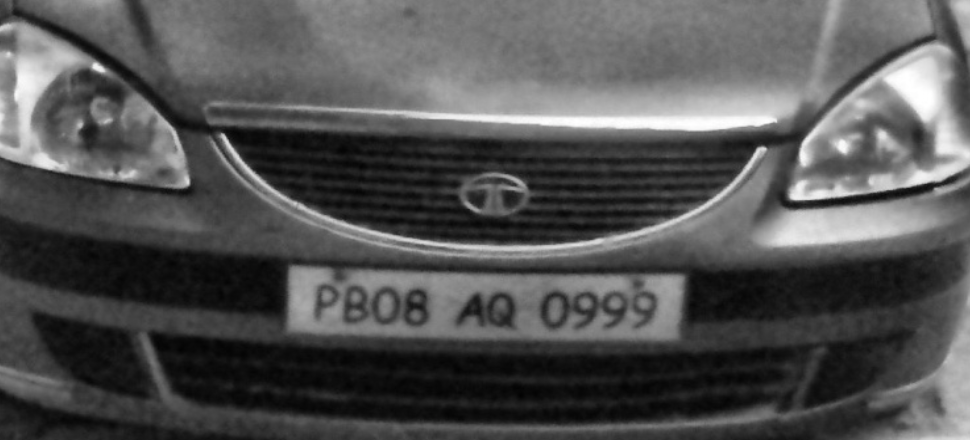
\includegraphics[width=88mm]{ext04.png}
	\caption{Aumento de contraste usando equalização de histograma adaptativo}
Fonte: An efficient approach for number plate extraction from vehicles image under image processing~\cite{kaur2014efficient}
	\label{fig:ext_contrast_adaptive_histogram}
\end{figure}

\subsection{Operações Morfológicas de Abertura e Subtração de Imagem}

A operação de abertura morfológica é realizada na imagem de escala de cinza
aumentada de contraste usando um elemento de estrutura em forma de disco. Na
subtração de imagem, a imagem morfológica aberta é subtraída da imagem de escala
de cinza aumentada de contraste.

\begin{figure}[H]
	\centering
	
\includegraphics[width=88mm]{ext05.png}
	\caption{Efeito de abertura}
Fonte: An efficient approach for number plate extraction from vehicles image under image processing~\cite{kaur2014efficient}
	\label{fig:ext_opening_effect}
\end{figure}

\begin{figure}[H]
	\centering
	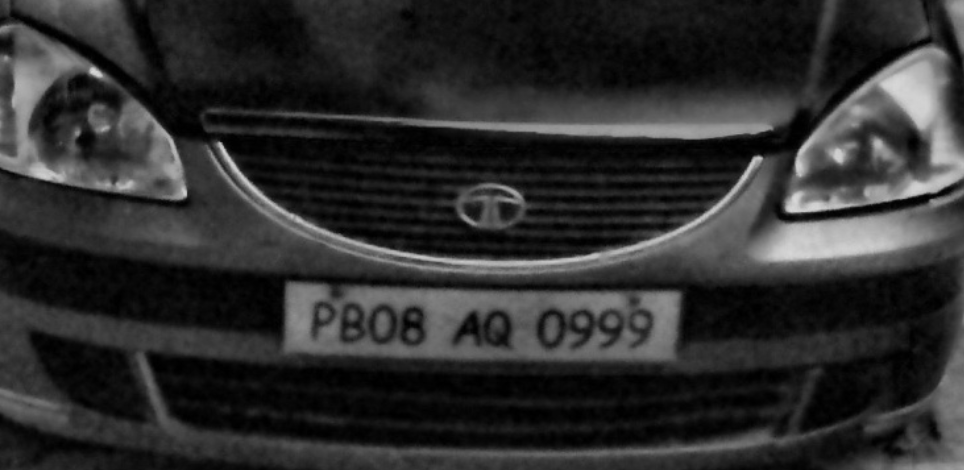
\includegraphics[width=88mm]{ext06.png}
	\caption{Imagem subtraída}
Fonte: An efficient approach for number plate extraction from vehicles image under image processing~\cite{kaur2014efficient}
	\label{fig:ext_image_substraction}
\end{figure}

\subsection{Binarização da Imagem}

Nesta operação a imagem de escala de cinza subtraída é convertida em imagem
binária. Em primeiro lugar, o nível de limiar é calculado pelo método de Otsu.
Tendo o limiar calculado, a imagem de escala de cinza subtraída é convertida em
imagem em preto e branco.

\begin{figure}[H]
	\centering
	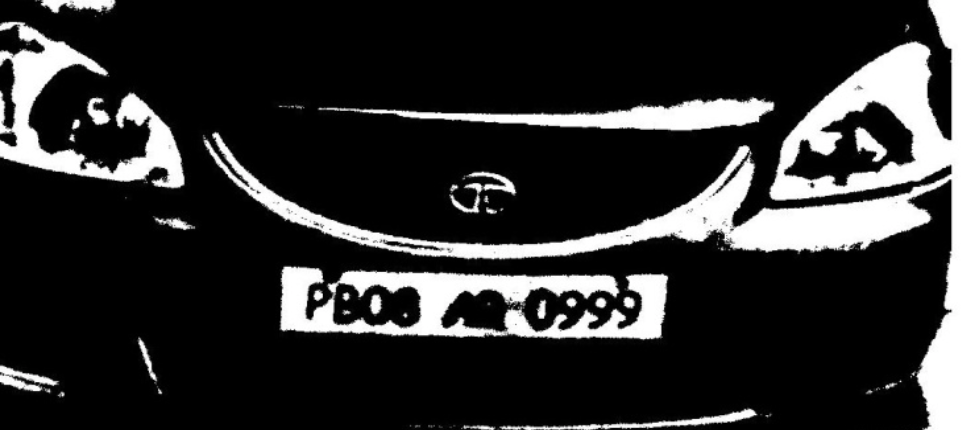
\includegraphics[width=88mm]{ext07.png}
	\caption{Imagem Binarizada}
Fonte: An efficient approach for number plate extraction from vehicles image under image processing~\cite{kaur2014efficient}
	\label{fig:ext_binarized_image}
\end{figure}

\subsection{Detecção de borda pelo operador Sobel}

A borda vertical é detectada pelo operador sobel e o resultado do operador sobel
ser aplicado à imagem binarizada é mostrado na figura~\ref{fig:ext_edge_detection_sobel}

\begin{figure}[H]
	\centering
	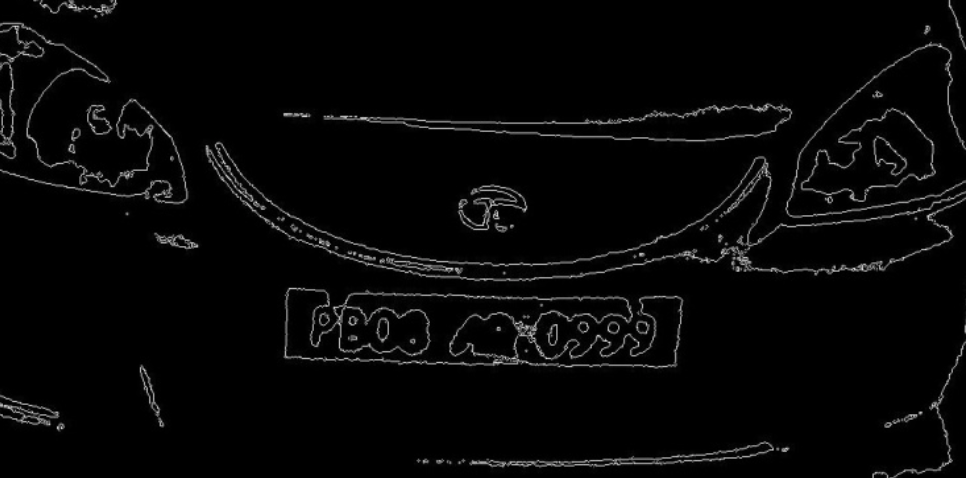
\includegraphics[width=88mm]{ext08.png}
	\caption{Detecção de borda pelo operador Sobel}
Fonte: An efficient approach for number plate extraction from vehicles image under image processing~\cite{kaur2014efficient}
	\label{fig:ext_edge_detection_sobel}
\end{figure}

\subsection{Detecção de Área de Placa Candidata por Operações Morfológicas de Abertura e Fechamento}

Com as operações morfológicas, os objetos indesejados na imagem são removidos.
Para a detecção da área da placa, uma operação de dilatação é aplicada na imagem
e depois os buracos são fechados. Em seguida, operações de abertura morfológica
e erosão são usadas para a detecção exata da área da placa.

\begin{figure}[H]
	\centering
	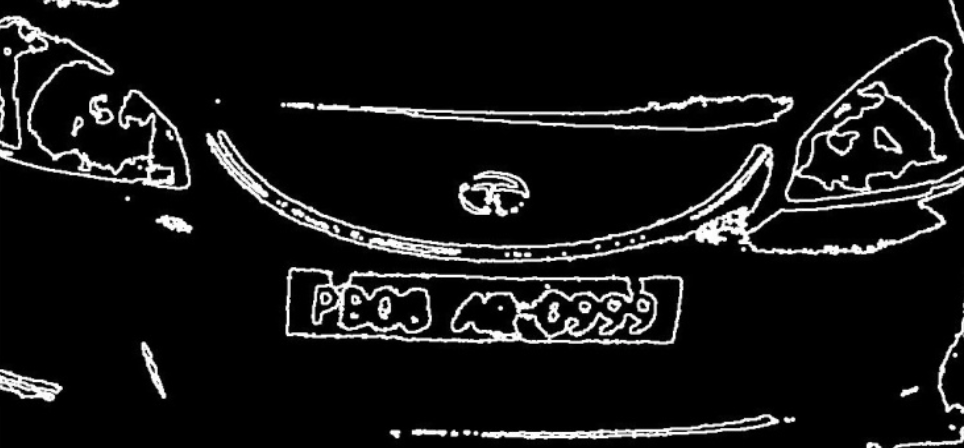
\includegraphics[width=88mm]{ext09.png}
	\caption{Dilatação morfológica}
Fonte: An efficient approach for number plate extraction from vehicles image under image processing~\cite{kaur2014efficient}
	\label{fig:ext_morphological_dilation}
\end{figure}

\begin{figure}[H]
	\centering
	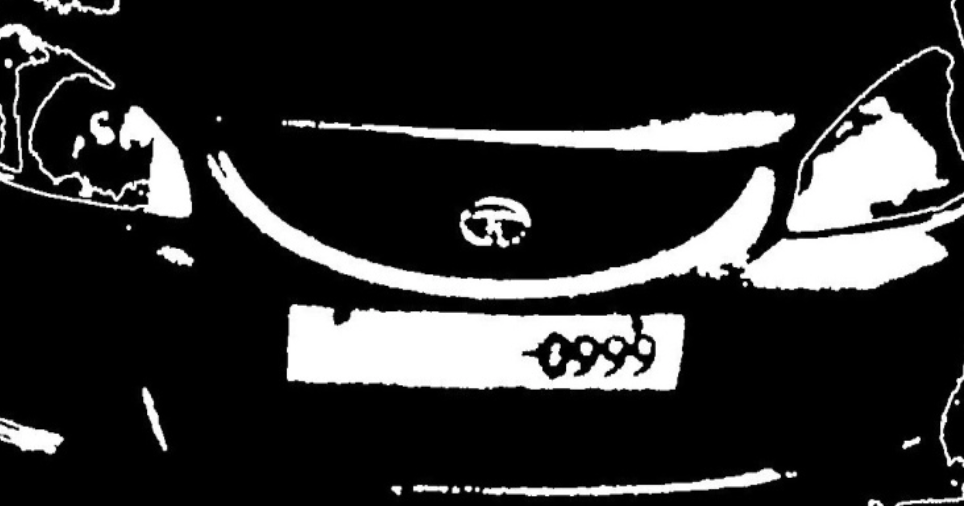
\includegraphics[width=88mm]{ext10.png}
	\caption{Após preenchimento dos buracos}
Fonte: An efficient approach for number plate extraction from vehicles image under image processing~\cite{kaur2014efficient}
	\label{fig:ext_holes_filled}
\end{figure}

\begin{figure}[H]
	\centering
	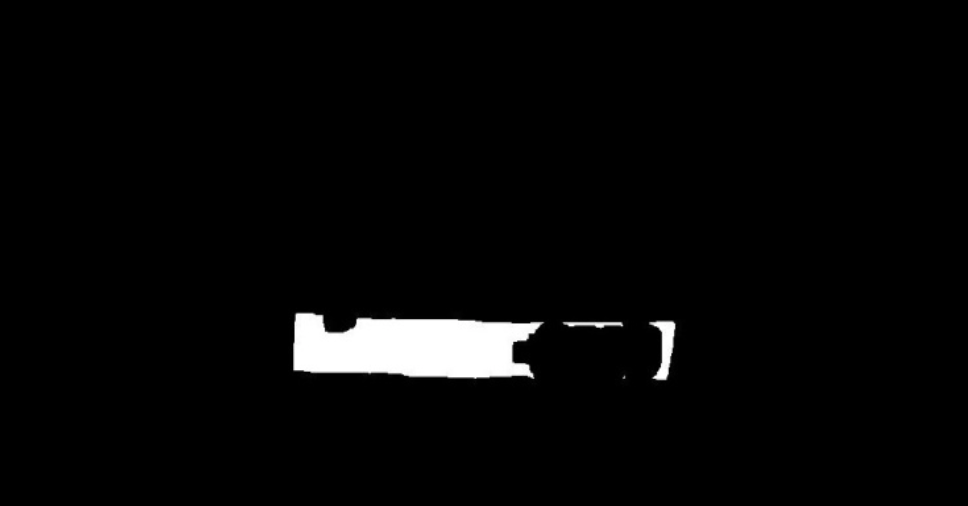
\includegraphics[width=88mm]{ext11.png}
	\caption{Detecção da área da placa}
Fonte: An efficient approach for number plate extraction from vehicles image under image processing~\cite{kaur2014efficient}
	\label{fig:ext_plate_area_detection}
\end{figure}

\subsection{Extração da área da placa real}

Após a detecção da área da placa, essa área é extraída da imagem. Em primeiro
lugar, os índices de linha e coluna da área da placa são encontrados por análise
de componentes conectados.

\begin{figure}[H]
	\centering
	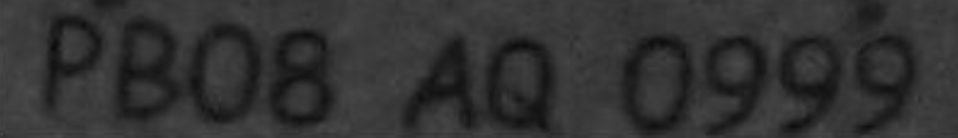
\includegraphics[width=88mm]{ext12.png}
	\caption{Placa extraída}
Fonte: An efficient approach for number plate extraction from vehicles image under image processing~\cite{kaur2014efficient}
	\label{fig:ext_true_number_plate}
\end{figure}

\subsection{Aprimoramento da região extraída}

A placa de número extraída pode consistir em vários ruídos ou furos indesejados.

\begin{figure}[H]
	\centering
	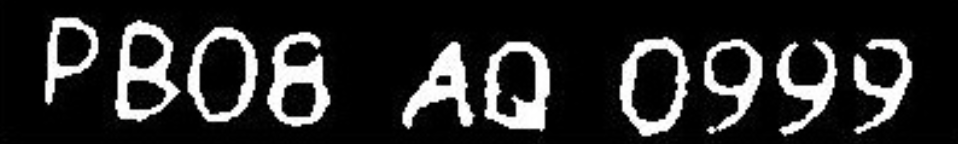
\includegraphics[width=88mm]{ext13.png}
	\caption{Placa aprimorada}
Fonte: An efficient approach for number plate extraction from vehicles image under image processing~\cite{kaur2014efficient}
	\label{fig:ext_enhanced_number_plate}
\end{figure}

\section{Segmentação dos caracteres}
\label{sec:segmentacao}

O terceiro passo para o reconhecimento da placa é a segmentação dos caracteres.
A segmentação dos caracteres consiste na extração dos caracteres utilizando
estratégias como projetar as suas informações de cores, rotulá-los ou comparar
suas posições com modelos. A placa extraída no passo anterior pode conter
problemas de inclinação ou iluminação, mas o algoritmo de segmentação deve
superar todos esses problemas com pré-processamento.~\cite{s2013automatic}

Badawy~\cite{s2013automatic} faz uma análise dos algoritmos de segmentação mais
utilizados com seus prós e contras.  Os principais algoritmos utilizados são:
segmentação utilizando conectividade de \emph{pixels}, segmentação utilizando
perfis de projeção, segmentação utilizando conhecimento anterior dos caracteres,
segmentação utilizando contorno dos caracteres e segmentação utilizando
características combinadas.

Analisando os resultados foi definido que a segmentação dos caracteres
utilizando perfis de projeção foi o mais eficiente, e que mais se encaixa no
problema proposto. Sanyuan~\cite{sanyuan2004car} utiliza essa técnica de
segmentação de caracteres, e, utilizando-a juntamente de remoção de ruídos e
análise de sequência de caracteres, obteve uma taxa de acerto de 99.2\% e uma
velocidade de processamento de 10 a 20 milisegundos, o que é bem animador. As
vantagens deste método são que a segmentação independe das posições dos
caracteres, e consegue lidar bem com rotações. Suas desvantagens são que é
afetada ruído na imagem e requer o conhecimento do número de caracteres na
placa, o que não será problema devido ao fato de as placas brasileiras terem um
número constante de caracteres.

Este método utiliza-se da diferença entre a cor dos caracteres da placa e a cor
do fundo da placa, por terem valores diferentes eles têm valores binários
opostos em uma imagem binária. Portanto, o método de segmentação consiste em
projetar a placa extraída verticalmente para determinar o início e final dos
caracteres e depois projetar os caracteres extraídos horizontalmente para
extrair cada caracter independente.

Badawy~\cite{s2013automatic} ainda afirma que é evidente que este método de
segmentação é o mais comum e o mais simples presente na literatura.

\section{Reconhecimento dos caracteres} \label{sec:reconhecimento}

O último passo para reconhecimento da placa é o reconhecimento ótico dos
caracteres extraídos. Os maiores desafios da extração de caracteres é o fato de
os caracteres extraídos não terem o mesmo tamanho e grossura, devido ao
\emph{zoom} da câmera. Outro problema, ao criar um reconhecedor de propósito
geral, é as diferentes fontes das diferentes placas ao redor do mundo.~\cite{s2013automatic}
Este segundo não será um problema para este trabalho pois
só há interesse em reconhecer placas brasileiras. Outro desafio é o
reconhecimento de caracteres semelhantes, como o D e o
0~\cite{ho2016intelligent}.  Esse problema será mitigado com o conhecimento
prévio das placas brasileiras, sabendo onde é possível haver letras e onde é
possível haver números.

Para o reconhecimento de caracteres foi escolhido utilizar o \emph{software}
\emph{Tesseract}. A ferramenta possui execução veloz e eficiente, permite o
treinamento para reconhecer novas fontes e suporte para diversas línguas.
